\documentclass{article}
\usepackage{amsmath}   % For math symbols and align environment
\usepackage{amssymb}   % For additional symbols
\usepackage{graphicx}  % For including figures

\begin{document}

\section*{A5}

\subsection*{(a)}

\textbf{F1 Results:}
\begin{itemize}
    \item Test Accuracy: \(0.9741\)
    \item Test Loss: \(0.0885\)
    \item Total Parameters: \(50,890\)
\end{itemize}

\begin{figure}[ht]
    \centering
    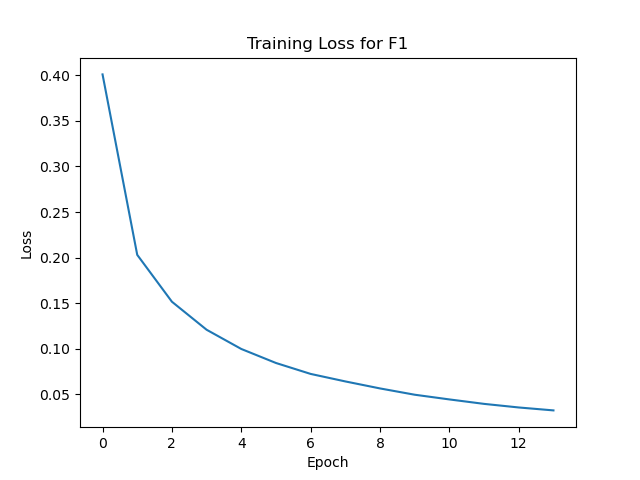
\includegraphics[width=0.75\linewidth]{F1_loss.png}
    \caption{Training loss versus epoch for the F1 model (shallow and wide).}
    \label{fig:f1_loss}
\end{figure}

\subsection*{(b)}

\textbf{F2 Results:}
\begin{itemize}
    \item Test Accuracy: \(0.9780\)
    \item Test Loss: \(0.0767\)
    \item Total Parameters: \(109,386\)
\end{itemize}

\begin{figure}[ht]
    \centering
    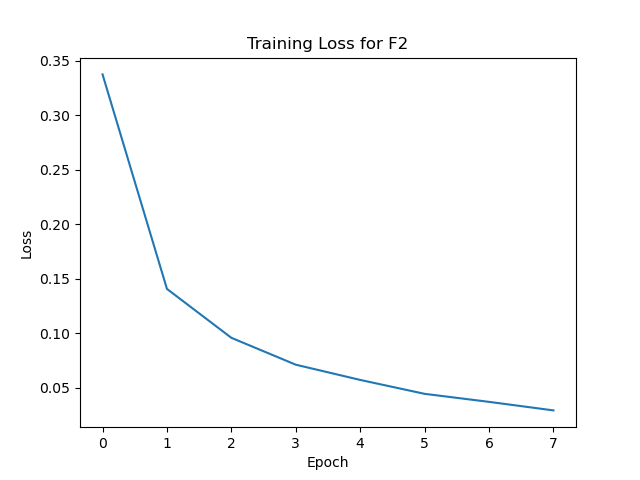
\includegraphics[width=0.75\linewidth]{F2_loss.png}
    \caption{Training loss versus epoch for the F2 model (narrow and deep).}
    \label{fig:f2_loss}
\end{figure}

\subsection*{(c)}
The F1 model, being shallow and wide, has fewer parameters (\(50,890\)) compared to the F2 model, which is deeper and narrower (\(109,386\)). Despite having fewer parameters, the F1 model achieves a high test accuracy of \(0.9741\), which is only slightly lower than the F2 model's test accuracy of \(0.9780\). 

The F2 model's deeper architecture allows it to capture more complex patterns in the data, which likely contributes to its slightly better performance. However, this comes at the cost of a significantly higher number of parameters, which increases the computational and memory requirements.

\end{document}
